\renewcommand{\theequation}{\theenumi}
\begin{enumerate}[label=\arabic*.,ref=\thesubsection.\theenumi]
\numberwithin{equation}{enumi}
\item total no of people working at the work place = 40
no of people live less than 7km from the work place = 9
let probability of a emgineer livinf less than 7 km from workplace = $P(<7)$
\begin{align}
P\left(X<7\right)&=\frac{9}{40}
\end{align}
\item no of people live more  than or equal 7km from the work place = 31
let probability of a emgineer livinf less than 7 km from workplace = $P(X \geq 7)$
\begin{align}
P\left(X \geq 7\right)&=\frac{31}{40}
\end{align}
\item there is no one who live within $\frac{1}{2}$ km from the work place so the probability will be 0.
\\
codes for the above equation can be get from here
\begin{lstlisting}
codes/prob/prob7.py
\end{lstlisting}
\begin{figure}[!ht]
	\centering
	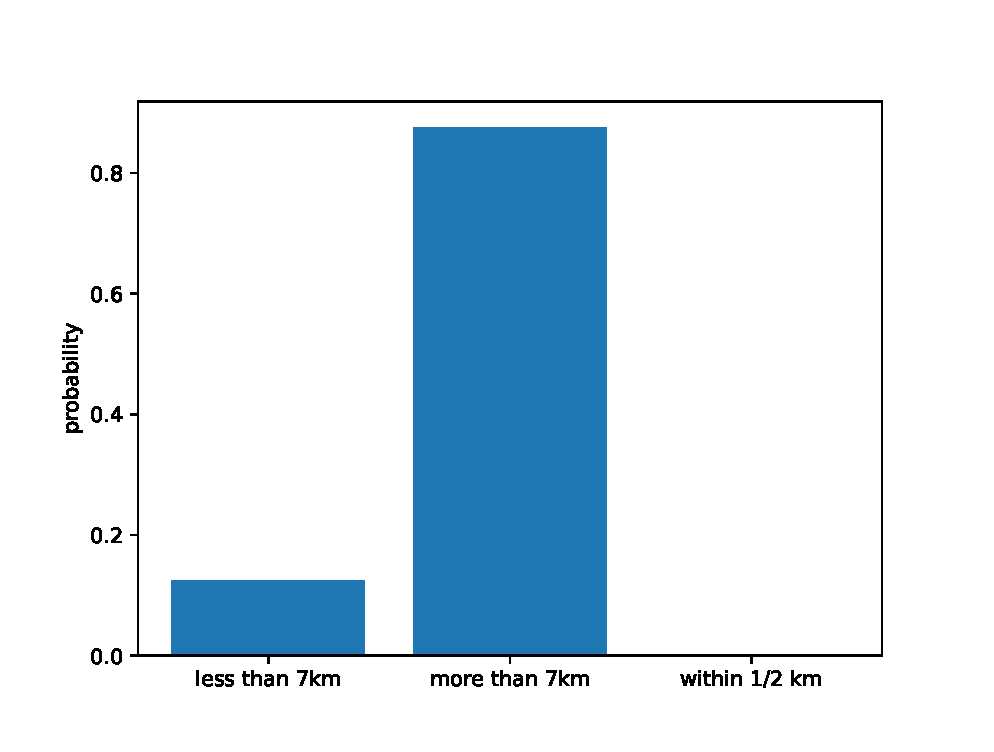
\includegraphics[width=\columnwidth]{./figures/prob/prob7.eps}
	\caption{probabilities a man to be near from work place}
	\label{fig:bt7}
	\begin{lstlisting}
	figs/prob/prob7.py
	\end{lstlisting}
\end{figure}
\end{enumerate}